\documentclass[onecolumn,10pt]{IEEEtran}
\usepackage{graphicx}
\usepackage{amsmath}
\usepackage{booktabs}
\usepackage{hyperref}
\renewcommand{\thetable}{S\arabic{table}}
\renewcommand{\thefigure}{S\arabic{figure}}
\renewcommand{\thesection}{S\arabic{section}}

\title{ChronoTrack: Supplementary Material}
\author{Surabhi Jagtap, Soheila Zeinali, Olivier Guenat, Tim Heinemann}

\begin{document}
\maketitle

This supplement reports the robustness, reproducibility, ablation and label-free analyses that support the main paper. Datasets, methods and notation are as in the main paper. The ARTORG dataset has four replicate wells (shown as mean $\pm$ SD); the Song et al.\ and Hachey et al.\ videos are not replicates and are shown one by one. The numbers behind every figure and table are provided as CSV files in the code repository (\texttt{paper/figure\_data}).

\section{Robustness and Reproducibility}
Because MVoC data have no ground truth, we test whether the features describe the chip rather than the processing (Fig.~\ref{fig:real}).

\emph{Missed detections:} we remove 5--30\% of the detections at random in every frame, re-run the whole pipeline (three repeats), and report the median relative change of the 13 features computed from the tracks. In the ARTORG dataset, the features change roughly in proportion to the loss ($33\pm3$\% at 30\% removed), in the Hachey et al.\ video less (12\%), and in the sparse Song et al.\ videos by 29--40\%. At the miss rates measured on the data (triangles), the change is at most 15\%. The miss rate is measured on isolated cells that stay in place: the fraction of such cells, found at the same spot in the frames before and after, that are missing in between.

\emph{Frame interval:} we keep only every $k$-th frame and recompute the features. Doubling the frame interval changes them by $17\pm5$\% in the ARTORG dataset (1 to 2\,h), 28--35\% in the Song et al.\ videos (5 to 10\,min) and 25\% in the Hachey et al.\ video (about 27 to 54\,min). Readouts should therefore only be compared at equal frame intervals.

\emph{Reproducibility:} for each feature, 100\% minus its coefficient of variation across the four ARTORG wells (100\%: the same value in every well; 0\%: a spread between wells as large as the mean). The on-vessel fractions of arrivals and departures (absolute and relative to chance), the track length and the departure rate are 94--98\% reproducible; the speeds and the extravasation and intravasation rates 77--87\%; the arrival rate 70\%; and the co-location of extravasation with regressing vessels, which builds on rare events, 59\%.

\begin{figure}[h]
    \centering
    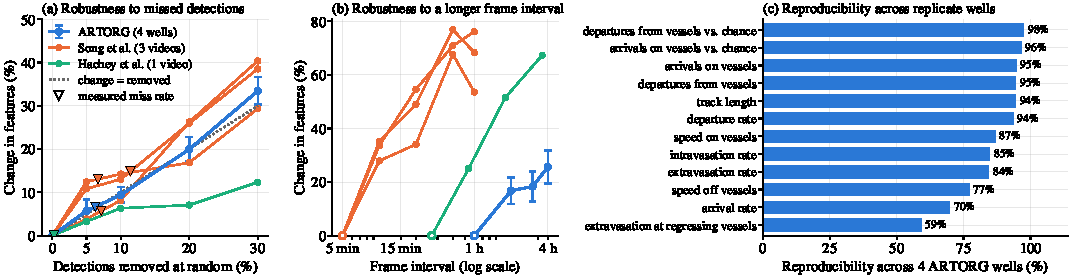
\includegraphics[width=\textwidth]{images/real_data.pdf}
    \caption{ChronoTrack on the three MVoC datasets (ARTORG: mean $\pm$ SD over four wells; Song et al., Hachey et al.: one line per video). (a) Relative change of the features when detections are removed at random (dotted: change equal to the fraction removed; triangles: miss rate measured on each sequence). (b) Relative change when only every $k$-th frame is used, against the resulting frame interval (open circles: native interval, estimated for Hachey et al.). (c) Reproducibility of each feature across the four ARTORG wells.}
    \label{fig:real}
\end{figure}

\section{Ablation on the Synthetic Twins}
Table~\ref{tab:ablation} compares ChronoTrack with four variants on the 48 synthetic twin sequences: forward frame-by-frame linking with the same cost terms and maximal gap (FbF), ChronoTrack with additional vessel cues (motion parameters on and off vessels, anisotropy along the vessel axis, distance to the vessel wall; +Vessel), a constant-velocity Kalman filter, and nearest-neighbor linking (NN). Frame-by-frame linking with the same cost terms comes within 0.1--0.4 F1 points of ChronoTrack and has similar complete-track fractions and feature errors; most of the gain over the published trackers therefore stems from the shared cost terms (persistent motion, bounded appearance cues, measured gap model), whereas time-symmetric optimization adds a small gain in accuracy and, above all, removes the dependence on the direction of time (Sec.~\ref{sec:labelfree}). Vessel cues change F1 by at most 0.2 points. The Kalman filter fails under ambiguous motion.

\begin{table}[h]
\centering
\caption{Ablation on the synthetic twins: median over the 12 sequences of a condition (4 wells $\times$ 3 seeds). $^{*}p<0.05$, $^{**}p<0.01$: difference from ChronoTrack (paired Wilcoxon signed-rank test, Holm-corrected over the 16 comparisons of a metric); ns: not significant. Feature error: lower is better.}
\label{tab:ablation}
\begin{tabular}{lccccc}
\toprule
Density, motion & ChronoTrack & FbF & +Vessel & Kalman & NN \\
\midrule
\multicolumn{6}{l}{\emph{Link F1 (\%)}} \\
Real, gentle & 97.5 & 97.4$^{*}$ & 97.5$^{**}$ & 95.7$^{**}$ & 94.6$^{**}$ \\
Real, ambiguous & 93.1 & 93.0$^{**}$ & 93.0$^{*}$ & 71.6$^{**}$ & 88.3$^{**}$ \\
2$\times$, gentle & 93.8 & 93.5$^{**}$ & 93.9$^{*}$ & 85.4$^{**}$ & 91.6$^{**}$ \\
2$\times$, ambiguous & 87.5 & 87.1~ns & 87.3~ns & 47.8$^{**}$ & 84.0$^{**}$ \\
\midrule
\multicolumn{6}{l}{\emph{Complete tracks (\%)}} \\
Real, gentle & 57.3 & 56.4~ns & 56.2$^{**}$ & 44.7$^{**}$ & 22.2$^{**}$ \\
Real, ambiguous & 26.1 & 26.2~ns & 25.3$^{*}$ & 4.9$^{**}$ & 8.5$^{**}$ \\
2$\times$, gentle & 29.7 & 29.6~ns & 29.3~ns & 14.0$^{**}$ & 11.9$^{**}$ \\
2$\times$, ambiguous & 9.3 & 9.4$^{*}$ & 8.9~ns & 0.7$^{**}$ & 4.0$^{**}$ \\
\midrule
\multicolumn{6}{l}{\emph{Feature error (\%)}} \\
Real, gentle & 3.0 & 3.1~ns & 3.3~ns & 5.9~ns & 8.0$^{**}$ \\
Real, ambiguous & 8.4 & 8.4~ns & 7.0~ns & 21.9$^{**}$ & 7.0~ns \\
2$\times$, gentle & 4.0 & 4.6~ns & 5.0~ns & 9.3$^{**}$ & 4.8~ns \\
2$\times$, ambiguous & 8.3 & 7.0~ns & 7.1~ns & 30.0$^{**}$ & 7.4~ns \\
\bottomrule
\end{tabular}
\end{table}

\section{Label-Free Tests on Real Data}\label{sec:labelfree}
\emph{Time reversal:} reversing a movie turns arrivals into departures, extravasation into intravasation and vessel regression into emergence. A tracker whose output does not depend on the direction of time should therefore map every event of the original movie onto its mirror event in the reversed movie. We count the events that lack it. ChronoTrack is lower than frame-by-frame linking in all eight sequences (paired Wilcoxon signed-rank test, $p=0.008$); its remaining mismatch arises because the descent finds a local minimum.

\emph{Broken tracks:} an arrival that follows a nearby departure within three frames suggests a track broken in two. We compare the frequency of such arrivals with the chance level expected from the density of departures (binomial test per sequence). They are rarer than chance in every ARTORG well and Song et al.\ video ($p<10^{-11}$), for both trackers, but more frequent in the Hachey et al.\ video with ChronoTrack (13\% vs.\ 1.8\%, $p<10^{-14}$), where touching cells in the forming network are merged into one detection.

\emph{Stationary cells:} isolated cells that did not move between consecutive frames should remain in one track; with ChronoTrack, they do in 98.3--100\% of cases in every sequence.

\begin{table}[h]
\centering
\caption{Label-free tests on real data for ChronoTrack (CT) and frame-by-frame linking with the same cost terms (FbF). ARTORG: mean $\pm$ SD over four wells; Song et al., Hachey et al.: per video. Broken tracks: arrivals within three frames after a nearby departure, observed / chance (\% of arrivals).}
\label{tab:labelfree}
\begin{tabular}{llccccc}
\toprule
 & & ARTORG & \multicolumn{3}{c}{Song et al.} & Hachey et al. \\
\cmidrule(lr){4-6}
Test & & 4 wells & S1 & S3 & S5 & \\
\midrule
Events without mirror (\%) & CT & 3.1$\pm$1.2 & 2.9 & 8.1 & 5.9 & 0.2 \\
 & FbF & 24.1$\pm$5.0 & 19.5 & 34.1 & 31.6 & 7.8 \\
Broken tracks, observed / chance (\%) & CT & 19$\pm$5 / 35$\pm$7 & 0 / 11.7 & 0.5 / 14.9 & 0.3 / 11.4 & 13.3 / 1.8 \\
 & FbF & 20$\pm$5 / 37$\pm$8 & 0 / 7.9 & 0 / 10.5 & 0.2 / 7.2 & 0 / 1.3 \\
Stationary cells kept in one track (\%) & CT & 99.0$\pm$0.5 & 99.3 & 99.6 & 99.6 & 100.0 \\
\bottomrule
\end{tabular}
\end{table}

\end{document}
